% SC2207 --- Chapter 6: Query Processing and Optimisation (0->100)
\chapter{Query Processing, Optimisation, and Cost Estimation}
\label{ch:query}

\begin{quote}
\emph{``Declarative in, procedural out---cost decides.''} You write what you want; the DBMS figures out how to get it fast by enumerating plans and picking the cheapest using statistics.
\end{quote}

\noindent\fbox{\parbox{\dimexpr\linewidth-2\fboxsep-2\fboxrule}{%
\textbf{From zero: algebra $\to$ execution.} We assume Ch.~2--3 (algebra, SQL, indexes) but no systems knowledge. Every operator and cost formula is motivated with a picture before symbols used.}}
\vspace{0.4em}

\section*{Learning Outcomes}
After this chapter you will be able to:
\begin{enumerate}[label=(L\arabic*)]
    \item outline the lifecycle parse $\to$ rewrite $\to$ optimise $\to$ execute;
    \item describe physical operators for selection, projection, join, and aggregation;
    \item estimate I/O and CPU cost using histograms and cardinalities;
    \item compare join algorithms (nested-loop, hash, sort-merge) by cost;
    \item read an EXPLAIN plan and spot a bad cardinality estimate.
\end{enumerate}

% ============================================================
\section{From Declarative Query to Execution Plan}
\label{sec:lifecycle}

\begin{figure}[h]
\centering
\begin{tikzpicture}[scale=0.73, every node/.style={font=\scriptsize},
  b/.style={draw, thick, rounded corners, align=center, minimum width=2.2cm, minimum height=0.70cm}]
  \node[b, fill=blue!12] (sql) at (0,3.0) {SQL text};
  \node[b, fill=green!12] (parse) at (0,2.15) {Parser + Resolver\\{\tiny algebra tree}};
  \node[b, fill=orange!15] (rewrite) at (0,1.30) {Rewriter\\{\tiny heuristic pushdown}};
  \node[b, fill=violet!12] (opt) at (0,0.45) {Cost-based optimiser\\{\tiny enumerate + pick cheapest}};
  \node[b, fill=red!12] (exec) at (0,-0.40) {Executor\\{\tiny volcano iterator}};
  \foreach \a/\b in {sql/parse, parse/rewrite, rewrite/opt, opt/exec} \draw[-{Stealth}, thick, blue!60!black] (\a)--(\b);
  \node[draw, thick, fill=yellow!10, rounded corners, inner sep=3pt, align=left, font=\tiny] at (5.2,1.30) {Statistics:\\$|R|$, $B(R)$,\\$V(A,R)$,\\histograms};
  \draw[-{Stealth}, thick, dashed, violet!60!black] (5.2,1.00) -- (0.95,0.45);
  \node[font=\tiny, fill=white, inner sep=1pt] at (3.6,0.85) {cost model};
\end{tikzpicture}
\caption{Query compilation pipeline. Rewriter applies algebra laws (Ch.~2); optimiser uses statistics to cost physical plans.}
\label{fig:pipeline}
\end{figure}

Parsing turns SQL into a logical algebra tree ($\sigma,\pi,\bowtie$). The rewriter applies equivalences: push selections past joins/projections, eliminate redundant subqueries, and flatten views. The optimiser then translates each logical operator to one or more physical operators and chooses the combination with lowest estimated cost. Finally the executor runs the chosen plan using an iterator (volcano) model: each operator implements \texttt{open--next--close} and pulls tuples on demand.

\subsection{Logical vs.\ Physical Operators}

Logical $\bowtie$ might become physical \emph{hash join}, \emph{sort-merge join}, or \emph{nested-loop join} depending on indexes, sizes, and predicates. Logical $\sigma$ might be an index scan vs.\ heap scan. This decoupling lets the optimiser explore dozens to thousands of plans for a single query.

% ============================================================
\section{Physical Operators and Their Costs}
\label{sec:physical}

We count page I/Os plus CPU per tuple; buffer hits are cheaper than misses but we estimate worst-case I/Os first. Let $B(R)$ be pages in $R$, $|R|$ tuples, $M$ buffer frames.

\paragraph{Selection $\sigma_{A=c}(R)$.} Heap scan $B(R)$ I/Os. B$^+$ on $A$: $h + \lceil\text{sel}\cdot|R|/ \text{rec/page}\rceil$ (clustered) or $h + \text{sel}\cdot|R|$ random for unclustered (may be worse than scan if selectivity high). Use index when selectivity low.

\paragraph{Projection $\pi$ with duplicate elimination.} Sort-based $O(B\log B)$ or hash-based $O(B)$; if an index already orders by the projection keys, a scan suffices. SQL without \texttt{DISTINCT} skips elimination.

\paragraph{Aggregation and GROUP BY.} Sort or hash partitioning; similar cost to projection.

\paragraph{JOIN is the expensive part.} Three families:

\begin{itemize}
    \item \textbf{Block nested-loop (BNL):} for each block of outer $R$ scan inner $S$. Cost $\approx B(R)+|R_{\text{blocks}}|\cdot B(S)$. Good when $S$ small or no index.
    \item \textbf{Index nested-loop:} for each $r\in R$ probe index on $S$. Cost $|R| \cdot (h+1)$ if index on join key. Wins when $R$ small and $S$ indexed.
    \item \textbf{Hash join (Grace):} partition both on hash of join key, then probe. Cost $\approx 3(B(R)+B(S))$ (partition+probe), linear. Best for large equi-joins without index.
    \item \textbf{Sort-merge join:} sort both (if not already sorted/index-ordered) then merge. Cost sort + $B(R)+B(S)$. Cheapest when inputs already sorted or output must be sorted.
\end{itemize}

\begin{figure}[h]
\centering
\begin{tikzpicture}[scale=0.71, every node/.style={font=\tiny},
  s/.style={draw, thick, minimum width=1.7cm, minimum height=0.65cm, align=center, rounded corners}]
  \node[s, fill=blue!12] (r) at (0,2.0) {Outer $R$\\scan blocks};
  \node[s, fill=orange!14] (hash) at (3.5,2.0) {Partition\\hash($key$)};
  \node[s, fill=green!14] (probe) at (3.5,0.7) {Probe HT\\with $S$};
  \node[s, fill=blue!12] (s) at (0,0.7) {Inner $S$\\scan / index};
  \node[s, fill=violet!12] (out) at (7.0,1.35) {Result\\$\bowtie$};
  \draw[-{Stealth}, thick] (r) -- (hash);
  \draw[-{Stealth}, thick] (s) -- (probe);
  \draw[-{Stealth}, thick] (hash) -- (probe);
  \draw[-{Stealth}, thick] (probe) -- (out);
  \draw[-{Stealth}, thick] (hash) -- (out);
  \node[font=\tiny, fill=yellow!10, draw, rounded corners, inner sep=2pt, align=left] at (7.0,0.05) {Hash: linear\\if $M$ large\\enough};
\end{tikzpicture}
\caption{Hash join dataflow. Partition phase splits both relations; probe phase emits matches without sorting.}
\label{fig:hash-join}
\end{figure}

\begin{example}[Choosing a join]
$|R|=10$k, $|S|=1$M, $S$ has B$^+$ on join key, $M=1000$. Index nested-loop: $10$k probes $\times$ $3$ I/Os = 30k. Hash join: $3(1$k+$10$k) $\approx$ 33k. BNL without index: far worse. Index NL wins.
\end{example}

\subsection{Other Physical Choices}

\emph{Sequential scan with prefetch} vs.\ \emph{index scan}; \emph{covering index} (index-only scan) avoids heap fetch; \emph{bitmap} intersection for multi-column ANDs. Sort for ORDER BY may reuse a merge-join's order.

\begin{example}[Covering index]
Query \texttt{SELECT code, avg(grade) FROM Enrolled WHERE code='SC2207' GROUP BY code} needs only \texttt{code} and \texttt{grade}. A B$^+$ on \texttt{(code,grade)} answers it from the index alone (index-only scan), saving the heap fetch per row---often $2\times$ faster.
\end{example}

\subsection{Pipelining vs.\ Materialisation}

Pipelined execution streams tuples operator-to-operator without writing intermediates to disk (volcano pulls). Blocking operators (\texttt{SORT}, \texttt{HASH BUILD}) must materialise before producing output. Pipelining saves I/Os but limits parallelism; optimisers weigh this via cost models with CPU and memory terms.

% ============================================================
\section{Cardinality Estimation and Histograms}
\label{sec:estimation}

Cost needs cardinalities. The catalog stores per table: $|R|$, $B(R)$, distinct values $V(A,R)$, min/max, and per column a \emph{histogram} (equi-width or equi-depth) and most-common-values list.

Estimate selectivity $\mathit{sel}$:
\begin{align*}
| \sigma_{A=c}(R)| &\approx |R|/V(A,R),\\
| \sigma_{A>c}(R)| &\approx |R|\cdot (\max -c)/(\max-\min),\\
|R\bowtie_{A} S| &\approx |R|\cdot|S|/\max(V(A,R),V(A,S))
\end{align*}
assuming uniform distribution and inclusion. Histograms refine range estimates: sum buckets up to $c$. Errors compound across joins---a bad histogram can mispredict by orders of magnitude, leading the optimiser to pick nested-loop over hash join catastrophically.

\begin{figure}[h]
\centering
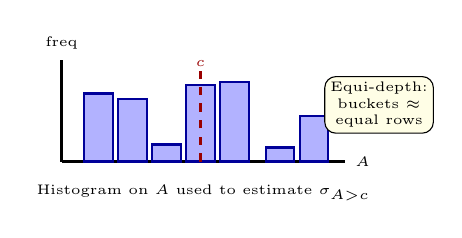
\begin{tikzpicture}[scale=0.72, every node/.style={font=\scriptsize}]
  \draw[thick] (0,0) -- (5.0,0) node[right, font=\tiny] {$A$};
  \draw[thick] (0,0) -- (0,1.8) node[above, font=\tiny] {freq};
  \foreach \x/\h in {0.4/1.2, 1.0/1.1, 1.6/0.3, 2.2/1.35, 2.8/1.4, 3.6/0.25, 4.2/0.8} {
    \draw[fill=blue!30, draw=blue!60!black, thick] (\x,0) rectangle (\x+0.5,\h);
  }
  \draw[thick, red!60!black, dashed] (2.45,0) -- (2.45,1.6) node[above, font=\tiny, fill=white, inner sep=1pt] {$c$};
  \node[font=\tiny, fill=yellow!10, draw, rounded corners, inner sep=2pt, align=center] at (5.6,1.0) {Equi-depth:\\buckets $\approx$\\equal rows};
  \node[font=\tiny, align=center] at (2.5,-0.55) {Histogram on $A$ used to estimate $\sigma_{A>c}$};
\end{tikzpicture}
\caption{Histogram buckets give piecewise-uniform estimate. Equi-depth handles skew better than equi-width.}
\label{fig:histogram}
\end{figure}

Keeping stats fresh (\texttt{ANALYZE}, auto-vacuum) and using extended stats (functional-dependency, n-distinct for multi-columns) are the cheapest optimisation you can do. When the optimiser is wrong, materialised CTEs or hints can pin a plan.

\begin{remark}[Correlated columns]
Independence assumption fails when columns correlate (e.g.\ \texttt{major} and \texttt{gpa} if CS curves differ). Multi-column histograms or learned estimators fix this; without them, $| \sigma_{\text{major=CS} \land \text{gpa}>4.0}|$ estimated as product of selectivities underestimates truth.
\end{remark}

\begin{example}[Estimation error propagation]
Three joins each mispredicted by $3\times$ yield $27\times$ total error. The optimiser may then choose a nested-loop that runs for minutes where a hash join finishes in seconds. EXPLAIN ANALYZE exposes the divergence row-by-row.
\end{example}

% ============================================================
\section{Plan Enumeration and EXPLAIN}
\label{sec:explain}

For $n$ joins, bushy vs.\ left-deep search spaces explode. Most optimisers use dynamic programming over subsets ($O(3^n)$) for $n\le10$--$12$ and greedy/heuristic beyond. They cost each subplan with the formulas above and keep the cheapest per interesting order.

\begin{lstlisting}[language=SQL, caption={Reading EXPLAIN}, label={lst:explain}]
EXPLAIN (ANALYZE, BUFFERS)
SELECT S.name, AVG(E.grade) FROM Student S
  JOIN Enrolled E ON S.id=E.studID
 WHERE S.major='CS' GROUP BY S.name;
-- Seq Scan on Student (cost=... rows=500 sel=0.2)
--  -> Hash Join (cost=... rows=8000)
--       -> Index Scan on Enrolled(code)
\end{lstlisting}

Look for: estimated rows vs.\ actual rows (ANALYZE), unexpected Seq Scans where an index exists, nested-loop with large outer, and spilled sorts (work\_mem exceeded). If estimated rows $\ll$ actual, the histogram is stale.

\begin{remark}[Parametric and adaptive]
Prepared statements reuse a plan for many parameter values; a plan optimal for selective $c$ may be terrible for unselective $c$ (parameter sniffing). Adaptive execution (re-optimise mid-flight, e.g.\ Spark AQE) mitigates this.
\end{remark}

\subsection{Heuristic Rewriting First}

Before costing, the rewriter applies cheap logical wins: push selections past joins (reduce input size early), push projections (trim width), eliminate redundant distinct, and unnest subqueries to joins where equivalent. These heuristics are always beneficial and shrink the DP search space, leaving the cost-based stage to choose among already-sensible plans.

\begin{example}[Unnesting]
\texttt{SELECT * FROM R WHERE R.a IN (SELECT S.a FROM S WHERE S.b=5)} rewrites to \texttt{R $\bowtie$ $\sigma_{b=5}(S)$} when $S.a$ is a key, enabling a hash join instead of a correlated nested loop---often $10\times$ faster.
\end{example}

\begin{remark}[Interesting orders]
If a later operator needs sorted output (\texttt{ORDER BY}, \texttt{GROUP BY}, merge join), preserving order early can avoid a final sort. Optimisers keep the cheapest plan \emph{per order} (``interesting orders'') to capture this trade-off, not just the globally cheapest.
\end{remark}

% ============================================================
\section{Chapter Notes}

System R (Selinger et al., 1979) pioneered cost-based optimisation with DP and the formulas above; Volcano/Cascades generalised enumeration. Reading: Garcia--Molina Ch.~16, Neumann et al.\ on adaptive joins. Modern cloud optimisers add learned cardinalities and materialised-view rewriting.

% ============================================================
\section{Exercises}
\label{sec:ch06-ex}
\begin{enumerate}[label=E6.\arabic*, leftmargin=*, itemsep=0.75em]
    \item \textbf{Warm-up: costs.} $B(R)=1000$, $B(S)=500$, $V(A,R)=100$, $V(A,S)=500$. Estimate $|\sigma_{A=5}(R)|$ and $|R\bowtie_A S|$. Recalculate if $A$ uniform vs.\ histogram showing $A=5$ is 5$\times$ average frequency.
    \item \textbf{Join choice.} Using BNL, index-NL ($h=3$), and Grace hash costs, pick the cheapest for $|R|=50$k ($B=500$), $|S|=500$k ($B=5000$), index on $S.A$ present, $M=100$. Show working.
    \item \textbf{Pushdown.} Prove $\sigma_{p(R)} (R\bowtie S)\equiv \sigma_{p}(R)\bowtie S$ when $p$ mentions only $R$. Draw the rewriter's transformation and explain why pushed plans are usually cheaper.
    \item \textbf{Histograms.} Construct equi-depth (3 buckets) for column values $[1,1,1,2,5,5,9,20]$. Estimate count for \texttt{WHERE $A$ BETWEEN 2 AND 6} via histogram vs.\ uniform; which is closer to truth?
    \item \textbf{EXPLAIN drill.} Given a plan showing Hash Join with estimated rows $10\times$ actual and a 2\,GB spill, propose two fixes (stats, memory, or rewrite) and predict each fix's cost effect.
    \item \textbf{Interesting orders.} Query \texttt{SELECT * FROM R JOIN S ON R.a=S.a ORDER BY R.a} may benefit from sort-merge join even if hash join is slightly cheaper. Explain why preserving sort order can dominate the trade-off.
\end{enumerate}
% End of Chapter 6
\relax % padding
\relax % padding
